
\section{复习}
\courseTime{Oct 24}
% 2022-10-24 07:59:36  Wenbin Fan @FDU
\chat{%
是人变少了吗,还是坐后面去了(笑)。

我们今天有节习题课,下周讲氢原子,慢慢接近于真实体系了,后面会安排上机,把我们的超算给同学们用。

今天要把上次课讲完,同时补充一些前面的内容。下午两节课习题课,助教来上。
}

上周课我们讲了转动角动量。

\chat{%
二维体系的时候,粒子在环形圆上运动,相当于势函数的边界条件跟 $r$ 能更好地分离变量,所以要做坐标变换,最关键的是动能部分的坐标变换。通过变换动能,得到了分离变量的哈密顿量。势函数是 delta 函数,因此哈密顿量跟自由粒子是一样的。

哈密顿量变换后,因为径向不变,其中对径向的偏导为 0,所以哈密顿量之跟角度有关。转动惯量定义为 $I = mr^2$。由周期性边界条件,得到了磁量子数。

随后定义了角动量,特别是 $z$ 轴的角动量。
由于 $l_z$ 对易,可以构造共同的本征函数完备集,
方向性可以体现在 $m$ 的正负上。一维拓展到三维。

对于球面上的粒子,与圆环上的粒子类似,势能只与 $r$ 有关,一样要做坐标变换。动能算符,其中的转动部分含有角度分量。二维中,$xOy$ 平面的角度是 $\theta$,三维中,角动量与 $z$ 轴的夹角是 $\theta$。

% $\hat L^2$ 的
第一次涉及到两个变量耦合的求解,成功地分离变量。

我们对勒让德方程做变换,是为了利用数学物理方程中的结论,更方便地求解。勒让德方程已经被研究得非常透彻。我们不是数学系、物理系,但鼓励学习数学物理方程、泛函分析等。
比如,导出薛定谔方程,需要有强大的数学直觉,我们现在学习也是为了以后寻找物理规律。
}

上节课讲到了\boldtext{幂级数展开},继续讲。勒让德方程里有一阶、二阶偏导,
\begin{align}
    H(x) = \sum_{j=0}^{\infty} a_j x^j, \quad H'(x) = \sum_{j=1}^{\infty} j a_j x^{j-1}, \quad H''(x) = \sum_{j=2}^{\infty} j(j-1) a_j x^{j-2},
\end{align}
得到了等间隔的递推公式
\begin{align}
    \sum_{j=1}^\infty
    \left\{
        (j+2)(j+1) a_{j+2} + \left[
            (j+ |m_l|)(j+ |m_l| +1) - M^2
        \right]a_j
    \right\} x^j = 0,
    % 2022-10-24 08:20:05  Wenbin Fan @FDU
\end{align}
若 $H(x)$ 是无穷级数,则 $H(x)$ 不是品优波函数。
所以,如果 $a_j$ 在 $k$ 截断,意味着这一项为 0,
\begin{align}
    a_{j+2} = \frac{(j+|m_l|)(j+|m_l|+1) - M^2}{(j+2)(j+1)} a_j,
\end{align}
参考 H. Eyring, J. Walter, Quantum Chemistry, \S 4. 

这里省略一些通用的推导。若 $H(x)$ 是无穷级数,则 $H(x)$ 不是品优波函数,当 $a_j$ 在 $k$ 截断,
\begin{align}
    (k+|m_l|)(k+|m_l|+1) - M^2 = 0, 
\end{align}
令 $l \equiv k + |m_l|$,则
\begin{align}
    M^2 = l(l+1),
\end{align}
其中
\begin{align}
    |m_l| = 0,1,2,\cdots, \quad l = 0,1,2,\cdots,
\end{align}
显然可知 $|m_l|_{\mathrm{max}} = l$。

% 2022-10-24 08:24:28  Wenbin Fan @FDU
再回到能量的量子化,体系的能量
\begin{align}
    - \frac{\hbar^2}{2m R^2} \hat\Lambda^2 Y(\theta, \varphi) = E Y(\theta, \varphi), 
    \label{eq:LambdaYEY}
\end{align}
分离变量得到
\begin{align}
    \hat \Lambda^2 \Theta(\theta) \Phi(\varphi) + M^2 \Theta(\theta) \Phi(\varphi)  = 0,
\end{align}
其中
\begin{align}
    M = E \frac{2mR^2}{\hbar^2} = \frac{2IE}{\hbar^2},
\end{align}
得到了能量的量子化
\begin{align}
    E = \frac{\hbar^2}{2I} \, l (l+1), \quad l = 0,1,2,\cdots,
\end{align}
与此同时,如果找到二者共同的本征函数,一定会有本征角量子数,并且角量子数 $m_l = 0, \pm1, \pm2, \cdots, \pm l$。

因为哈密顿算符 $\hat H$ 和 $l_z$ 是对易的。如果取二者共同的本征函数,
两个算符作用上去,
就会有两个量子数 $m_l$ 和 $l$,这也就是为什么把 \eqref{eq:LambdaYEY} 写成
\begin{align}
    - \frac{\hbar^2}{2I} \hat\Lambda^2 Y_{l,m_l}(\theta, \varphi) = \frac{\hbar^2}{2I} l(l+1) Y_{l,m_l}(\theta, \varphi). 
\end{align}
我们知道 $\hat \Lambda$ 和 $\hat L$ 是等价的,$\hat L^2 = -\hbar^2\hat L^2$,那么代入这个等式,有
\begin{align}
    \frac{1}{2I} \hat L^2 Y_{l,m_l}(\theta, \varphi) &= \frac{\hbar^2}{2I} l(l+1) Y_{l,m_l}(\theta, \varphi) \\
    \hat L^2 Y_{l,m_l}(\theta, \varphi) &= \hbar l (l+1) Y_{l,m_l}(\theta, \varphi)\label{eq:6_l_squared}
\end{align}
很自然地给出了角动量算符在三维体系中的本征函数。

后面求氢原子体系,当然要做一些额外的坐标变换,其势能函数只与径向有关(库伦算符),角度部分是球谐形式,所以我们求解的也是氢原子的角度部分。

\eqref{eq:6_l_squared} 中也能推导出 $z$ 方向的本征值,
\begin{align}
    \hat L_z = -\ii\hbar \pdv{\varphi} \Rightarrow \hat l_z Y_{l,m_l}(\theta, \varphi) = m_l Y_{l,m_l}(\theta, \varphi), 
\end{align}
\begin{align}
    |m_l|_{\mathrm{max}} = l, \quad \langle \hat l_z \rangle^2 |_{\mathrm{max}} = l^2, 
    \quad \langle \hat L^2 \rangle = l(l+1),
\end{align}
$z$ 方向一定有不确定性,类似于零点能。
% 【】一定会留下一份。
% 讲错了
% 2022-10-24 08:35:49  Wenbin Fan @FDU
也可以理解成「测不准原理」。
\begin{figure}
    \centering
    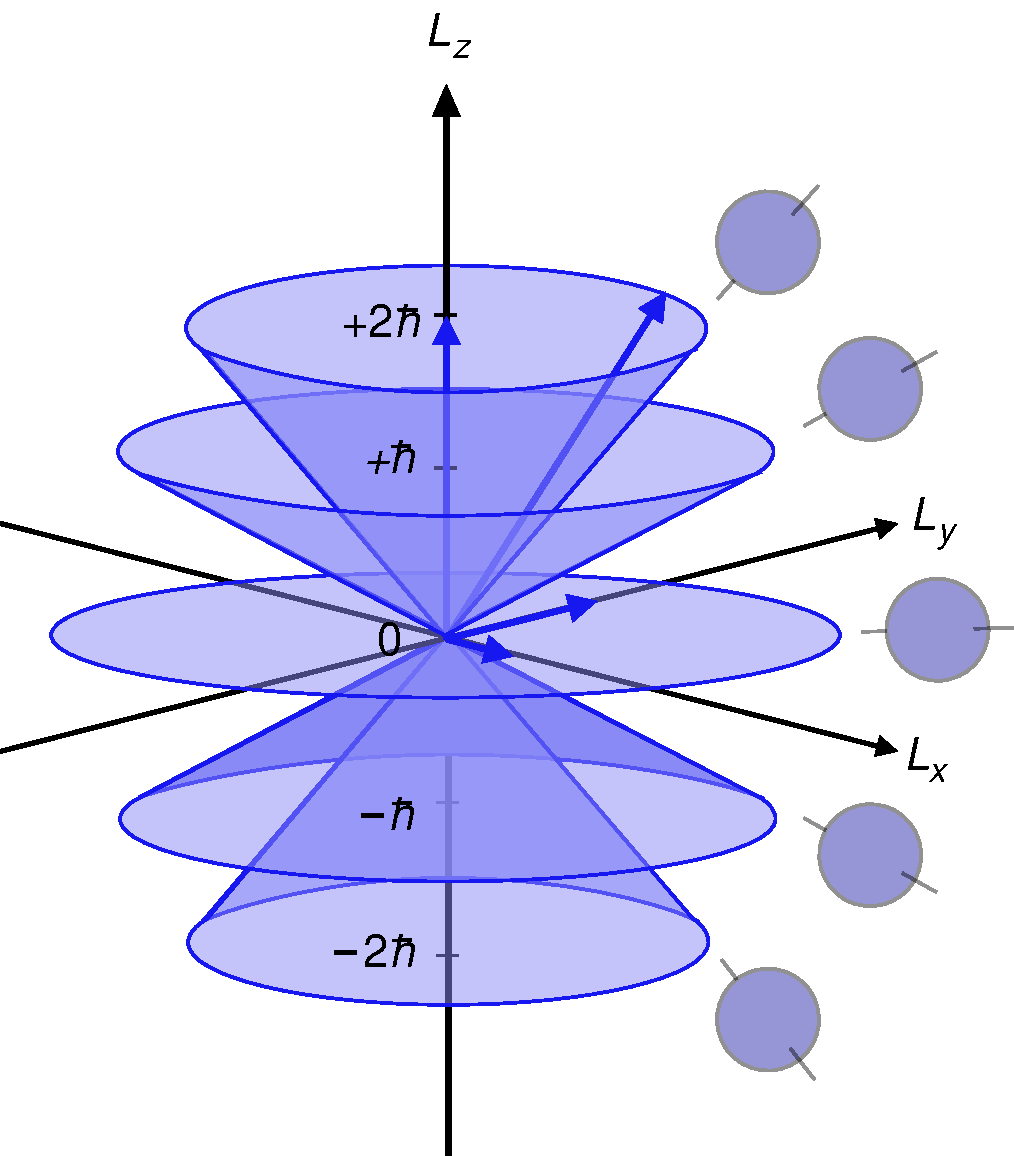
\includegraphics[height=3cm]{fig/angular_momentum_Wikipedia.pdf}
    \caption{角动量量子化}
\end{figure}

\homework{
    \textbf{6.1}  对于一个电子 $m_{\mathrm e} = \SI{9.11E-31}{\kilo\gram}$,以及一个陀螺 $m = \SI{0.02}{\kilo\gram}$,如果转动半径均为 $r = \SI{1.0}{\centi\metre}$,且运动速度均为 $\SI{1}{\metre\per\second}$,求被允许的角动量的最小 $\theta$ 值。
}
% % 2022-10-24 08:39:03  Wenbin Fan @FDU
% 我们已经有了能量量子化的讨论。能量量子化不仅引出了角动量的量子化,还有 $z$ 方向最小为 1 的不确定性。有意思的是,如果角量子数越来越大,不确定性的分量越来越小。

\subsection{体系的波函数}
已知
\begin{align}
    H(x) = \sum_{\substack{j=1,3,5,\cdots \\\text{or } 2,4,6,\cdots}}^{l-|m_l|} a_j \lambda^j \Rightarrow y(x) = (1-x^2)^{|m_l|/2} \sum_{\substack{j=1,3,5,\cdots \\\text{or } 2,4,6,\cdots}} a_j x^j, 
\\
    \Rightarrow \Theta_l^{m_l} (\theta) = (\sin\theta)^{|m_l|} \sum a_j (\cos\theta)^j
\end{align}
代回到球谐函数中,经过推导,有
\begin{align}
    Y_{l,m_l}(\theta) 
    % &= \Theta_m^{m_l} (\theta) \Phi_{m_l}(\varphi) \\
    &= A (\sin\theta)^{|m_l|} 
    \sum_{\substack{j=1,3,5,\cdots \\\text{or } 2,4,6,\cdots}}^{l-|m_l|}
    a_j (\cos\theta)^j \ee^{\ii m_l \varphi} \\
    &= \left[
        \frac{(2l+1) (l-|m_l|)!}
        {4\pi(l+|m_l|)!}
    \right]^{1/2}
    P_l^{m_l}(\cos\theta) \ee^{\ii m_l \varphi},
\end{align}
其中的 $P$ 称为连带勒让德函数(连带 associated,勒让德 Legendre)。
% % 2022-10-24 08:44:27  Wenbin Fan @FDU
% % 2022-10-24 08:58:40  Wenbin Fan @FDU
% 经过非常复杂的推导,推出来
% \begin{align}
%     Y_{l,m_l} (\theta) = A [][][]
% \end{align}

这里略过了很多推导,因为确实非常复杂。如果要讲清楚,可能要往回查一百年的论文。数学家们,已经分析清楚了很多微分方程,包括它们的特征、极限等,有的微分方程甚至已经整理成表格供查阅。

% 2022-10-24 08:59:20  Wenbin Fan @FDU
当 $l=0$、$m_l = 0$,
\begin{align}
    Y_{00} = A a_0 = C (\text{常数}),
\end{align}
面积分为
\begin{align}
    &\phantom{=}\oiint |Y_{00}(\theta, \varphi)|^2 \dd S 
    = \oiint C^2 R^2 \sin\theta \dd\theta \dd\varphi\\
    &= C^2 R^2 \int_0^\pi \sin\theta \dd\theta \int_0^{2\pi} \dd\varphi \\
    &= 4 \pi C^2 R^2 = 1, 
\end{align}
得到
\begin{align}
    C = \frac1{\sqrt{4\pi R^2}} = \frac1{\sqrt S},
\end{align}
其中的 $S$ 是球的表面积。
密度
\begin{align}
    \rho_{00}(\theta, \varphi) = C^2 = \frac1S,
\end{align}

当 $l=1$、$m=\pm1$ 时,
\begin{align}
    Y_{1,\pm1}(\theta, \varphi) = A a_0 \sin\theta \ee^{\pm\ii\varphi} = C \sin\theta \ee^{\pm\ii\varphi},
\end{align}
密度
\begin{align}
    \rho_{1,\pm1} (\theta, \varphi) = C^2 \sin^2\theta, 
\end{align}
面积分
\begin{align}
    \oiint \rho_{1,\pm1} (\theta, \varphi) \dd S 
    &= C^2 R^2 \int_0^\pi \sin^3\theta \dd\theta \int_0^{2\pi} \dd\varphi \\
    &= 2\pi c^2 R^2 \int_0^\pi \sin^3\theta \,\dd\theta,
\end{align}
利用积分变换
\begin{align}
    \dd\theta = \dd\cos\theta \frac{\dd\theta}{\dd\cos\theta} = -\frac{1}{\sin\theta} \dd\cos\theta,
\end{align}
则面积分继续推导
\begin{align}
    &= 2\pi C^2R^2 \int_1^{-1} (-\sin^2\theta)\dd\cos\theta \\
    &= 2\pi C^2R^2 \int_{-1}^{1} \sin^2\theta\,\dd\cos\theta \\
    &= 2\pi C^2 R^2 \int_{-1}^1 (1-\cos^2\theta) \dd\cos\theta\\
    &= \frac83 C^2R^2 = 1
\end{align}
解得
\begin{align}
    C^2 = \frac 38 \frac1{\pi R^2} = \frac 32 \frac1S \Rightarrow C = \sqrt{\frac32}\frac1{\sqrt S}. 
\end{align}

% 2022-10-24 09:14:29  Wenbin Fan @FDU
\chat{%
与化学体系挂钩,离域电子、拓扑材料等,拓扑超导实在材料的边缘,这里的电子一旦能够超导,电子就形成了新的量子化条件,本质就是环形或方形或球形的条件,求解它就会有些有意思的解出现。

第二部分是圆上和球上的电子,探讨了坐标变换,引入了角动量算符,为求解氢原子体系打下了基础。氢原子中,一旦变成了极坐标的形式,角度部分没有意外就是这种形式,我们到时会更关注径向部分。

我们到现在就讲完了,那么我们可以回头补一下以前没讲清楚的内容,比如是跟实验相关的。

}

\section{有限高方势垒}

\chat{%
我们补充一下有限高方势垒,像什么模型?(安静……)很像能垒嘛,比如物化中的热力学控制平衡、动力学控制快慢,进而调控反应选择性。催化不改变反应物、产物,热力学性质不能变,只能变动力学性质,即能垒的高度,高度直接决定了反应的快慢。

这个方形势垒特别像能垒。如果我们求解了方势垒,那么就能描述常见的平滑势垒。实际上,这个模型还特别像 STM 模型。通过电流大小,直接能探测到电子的密度。

按照之前的求解,首先要划分解的范围,低于 $V_0$ 称为束缚态,高于$V_0$是经典情况,我们关心的束缚态,即动量不足以使得粒子越过能垒的情况。
}

从薛定谔方程,可写出波函数,
\begin{align}
    \psi(x) = \begin{cases}
        C_1 \ee^{\ii k_1 x} + C_2 \ee^{-\ii k_1 x},\quad &x<0, \\
        C_3 \ee^{k_2 x} + C_4 \ee^{-k_2 x},\quad &0\leqslant x \leqslant l,\\
        C_5 \ee^{-\ii k_1 x}, \quad &x>l,
    \end{cases}
\end{align}
其中每一项都有其物理含义,如 $C_1$ 项表示往正向去的波,$C_2$ 项表示反射回的波,$C_3$、$C_4$ 表示透射波。

由概率流的概念,直接写出入射波、反射波、透射波的概率流密度,分别为
\begin{align}
    \frac{\hbar k}{m} |C_1|^2, \quad \frac{\hbar k}{m} |C_2|^2, \quad \frac{\hbar k}{m} |C_3|^2
\end{align}
定义反射系数和透射系数
\begin{align}
    &R = \frac{|C_2|^2}{|C_1|^2} = 
    \frac{(k_1^2 + k_2^2)^2 \sinh^2  k_2 l} {(k_1^2 + k_2^2) \sinh^2 k_2l + 4 k_1^2 k_2^2}, \\
    &T = \frac{|C_3|^2}{|C_1|^2} = 
    \frac{4 k_1^2 k_2^2} {(k_1^2 + k_2^2) \sinh^2 k_2l + 4 k_1^2 k_2^2},
\end{align}
二者满足 $R+T=1$。

当 $k_2l$ 足够大,即 $V_0 \gg E$,
\begin{align}
    \sinh^2 k_2l \approx \frac 14 \ee^{2k_2 l},
\end{align}
因为
\begin{align}
    \sinh^2 k_2 l = \left[\frac12\left(\ee^{k_2l} - \ee^{-k_2l}\right)\right]^2 = \frac14 \left(\ee^{2k_2 l} - 2 + \ee^{-2k_2 l}\right) \approx \frac 14 \ee^{2k_2 l},
\end{align}
这里忽略了比较小的常数 2 和很小的负指数。
代入 $k_2$、$k_3$ 的定义,有
\begin{align}
    T &\approx \frac{16 k_1^2 k_2^2}{(k_1^2 + k_2^2)^2} = \frac{16E(V_0 - E)}{V_0^2} \exp\left(\frac{2l}{\hbar}\sqrt{2m(V_0 - E)}\right) \\
    &\approx \frac{16 E}{V_0} \exp\left(\frac{2l}{\hbar}\sqrt{2m V_0}\right). 
\end{align}
在扫描隧道显微镜 scanning tunneling microscopy STM 中,电流 $I \propto \ee^{-2 k d}$,对比可知 $I \propto T$、$d\propto l$,$k$ 是与实验相关的常数。

STM 可以反映表面的形貌,有恒高、恒电流模式。

隧穿到底有多强?做个简单的练习。

对电子来说,设能垒的宽度 $\SI{1.0}{\angstrom} = \SI{1E-10}{\metre}$,设 $V_0 - E = \SI{5}{\electronvolt}$,那么
\begin{align}
    T &\propto \exp\left(-\frac{2l}{\hbar} \sqrt{2m(V_0 - E)}\right) \\
    &= \exp\left(
        - \frac{2\times\SI{1E-10}{\metre}}{\SI{1.05E-34}{\joule\second}}
        \sqrt{2\times\SI{9.11E-31}{\kilo\gram}\times\SI{5}{\electronvolt}}
    \right)
    \\ & = \ee^{-2.29} = 0.101
\end{align}
如果一个电子看到的势垒高度是 $\SI{5}{\electronvolt}$,它有 10\% 的概率可以隧穿过去。

对于原子来说,这个几率就小到了 $T\sim \ee^{-98.2} = \num{2.30E-43}$,基本不可能。

